\section{Experimental evaluation}\label{sec:experiment}
In this section, an experimental evaluation over X real-life event logs is reported.


\subsection{Re-sampling and test setup}
Time series are obtained by specifying a number of intervals (i.e. time steps in the DF series) using either equitemporal or equidistant aggregation.
Time series algorithms are parametric and sensitive to sample size requirements \cite{hanke2001business}.
Depending on the number of parameters a models uses a minimum size of at least 50 steps is not uncommon although typically model performance should be monitored at a varying number of steps.
In the experimental evaluation, 50 and 100 intervals will be used.

Three widely-used event logs are used (e.g. see []): the 2012 BPI challenge log\footnote{\url{https://doi.org/10.4121/uuid:3926db30-f712-4394-aebc-75976070e91f}}, the Sepsis cases event log\footnote{\url{https://doi.org/10.4121/uuid:915d2bfb-7e84-49ad-a286-dc35f063a460}}, and the Road Traffic Fine Management Process log\footnote{\url{https://doi.org/10.4121/uuid:270fd440-1057-4fb9-89a9-b699b47990f5}} (RTFMP) event log.
Each of these logs has a diverse set of chacteristics in terms of case and activity volume, as well as average trace length as can be seen in Table \ref{tab:eventlogs}.
\begin{table}[htbp]
  \centering
    \begin{tabular}{lrrr}
    \toprule
    \textbf{Event log} & \multicolumn{1}{l}{\textbf{\# cases}} & \multicolumn{1}{l}{\textbf{\# activities}} & \multicolumn{1}{l}{\textbf{Average trace length}} \\
    \midrule
    \textbf{BPI 12} & 13,087 & 36    & 20.020 \\
    \textbf{Sepsis} & 1,050 & 16    & 14.490 \\
    \textbf{RTFMP} & 150,370 & 11    & 3.734 \\
    \bottomrule
    \end{tabular}%
  \caption{Overview of the characteristics of the event logs used in the experimental evaluation.}
  \label{tab:eventlogs}%
\end{table}%

An example of applying the equisize or equitemporal aggregation to the event logs with 100 intervals results in the DF time series of Figures \ref{fig:bpi12ts} to \ref{fig:rtfmpts} where the most frequently and 50th most frequently occurring activity pairs are included.
The equitemporal aggregation is based on a number of intervals over the whole timespan of the event log.
When using this aggregation, a noticeable decline of DF pairs is visible towards the end of the series.
This phenomenom is typical in event logs, as processes typically have particular endpoint activity, e.g., the closure of a loan application event in the BPI 12 log.
The use of a cutoff of 50 for the most-frequently occurring DF pairs results in different time series as well.
For the BPI 12 log, the frequency of the 50th pair is still relatively high, while for the other event logs the frequency of the DF pair is low and close to 0, making the series unsuitable for analysis with white noise series analysis techniques that assume stationarity.
Ideally, every time series is tested using a stationairty test such as the Dickey-Fuller unit root test \cite{leybourne1995testing} and establish an appropriate lag order for differencing. 
Furthermore for each algorithm, especially ARIMA-based models, (partial) autocorrelation could establish the ideal $p$ and $q$ parameters.
However, for the sake of simplicity and to avoid tedious solutions where each activity pair has to have different parameters, various values are used $p$, $d$, and $q$ and applied to all DF pairs where only the best-performing are reported below for comparison with the other time series techniques.

\begin{figure}[tb]
	\centering
	\subfigure[Most common DF - equisize]{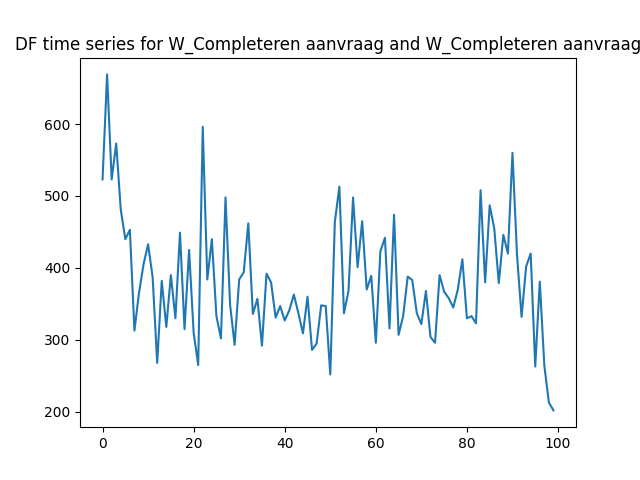
\includegraphics[width=0.49\textwidth]{./img/bpi12_1.png}}
	\subfigure[50th most common DF - equisize]{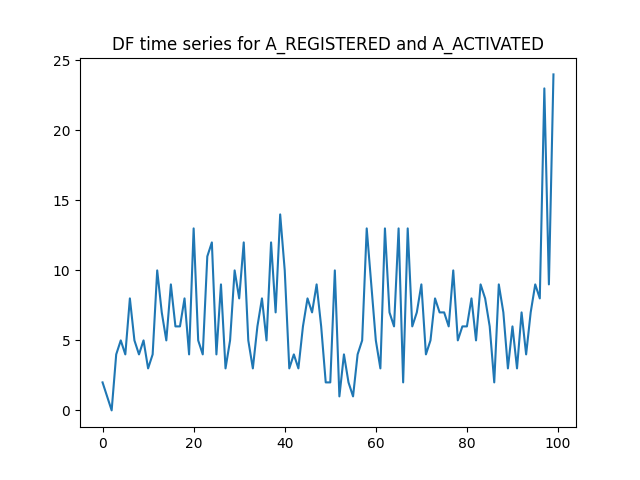
\includegraphics[width=0.49\textwidth]{./img/bpi12_2.png}}
	\subfigure[Most common DF - equitemp]{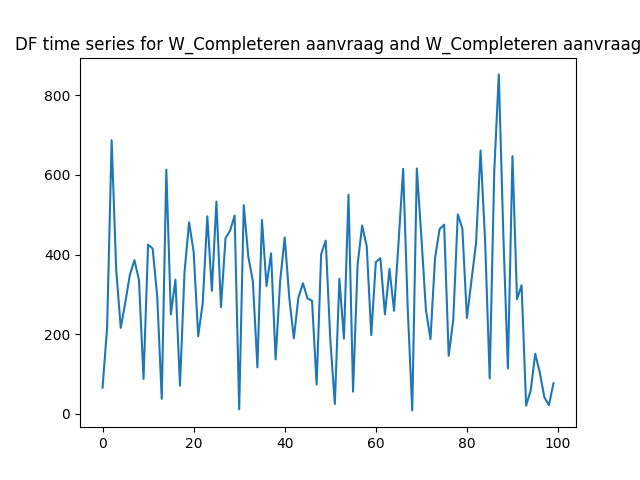
\includegraphics[width=0.49\textwidth]{./img/bpi12_1_t.png}}
	\subfigure[50th most common DF - equitemp]{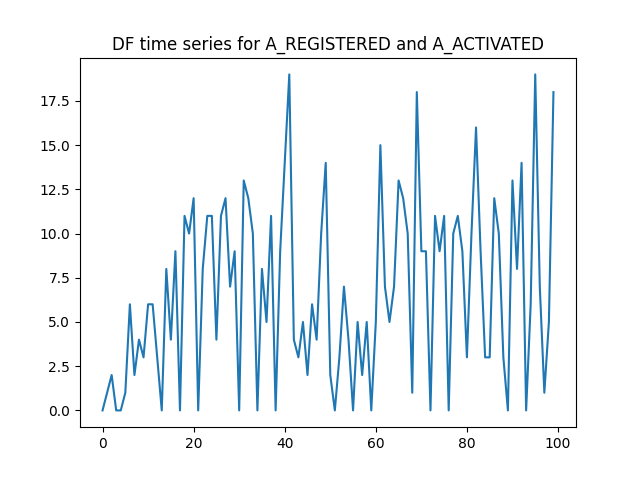
\includegraphics[width=0.49\textwidth]{./img/bpi12_2_t.png}}
	\caption{BPI 12}
	\label{fig:bpi12ts}
\end{figure}

\begin{figure}[tb]
	\centering
	\subfigure[Most common DF - equisize]{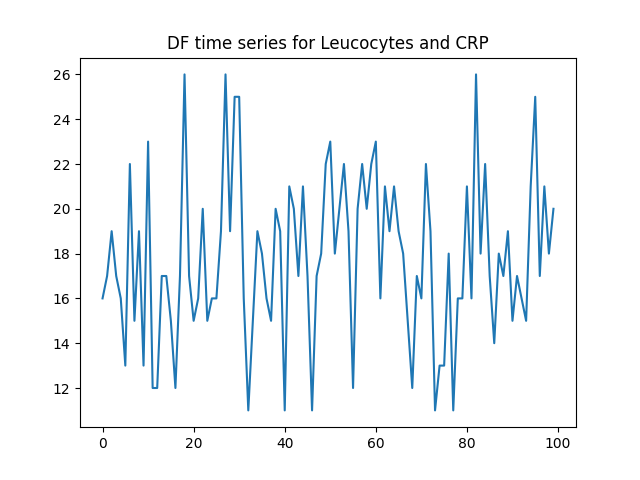
\includegraphics[width=0.49\textwidth]{./img/sepsis_1.png}}
	\subfigure[50th most common DF - equisize]{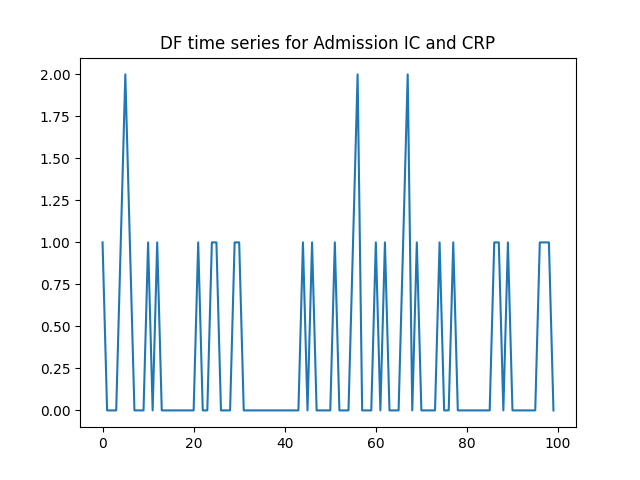
\includegraphics[width=0.49\textwidth]{./img/sepsis_2.png}}
	\subfigure[Most common DF - equitemp]{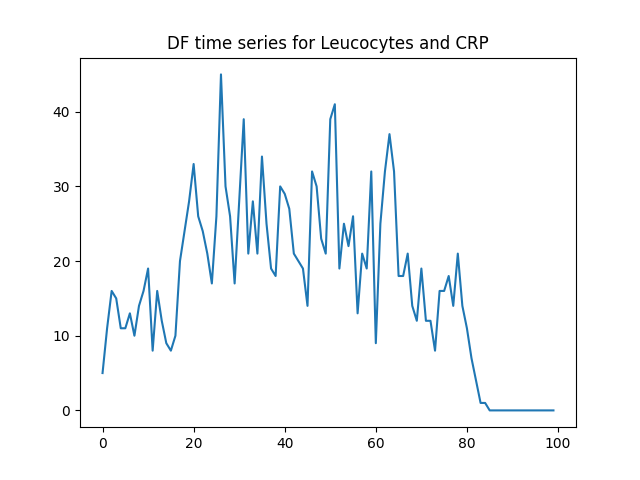
\includegraphics[width=0.49\textwidth]{./img/sepsis_1_t.png}}
	\subfigure[50th most common DF - equitemp]{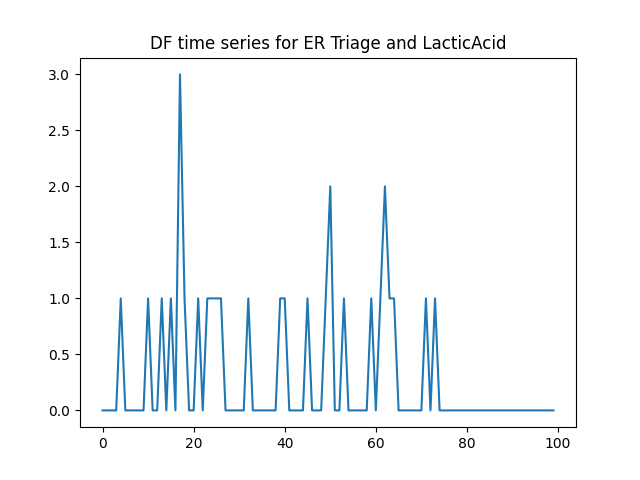
\includegraphics[width=0.49\textwidth]{./img/sepsis_2_t.png}}
	\caption{Sepsis}
	\label{fig:sepsists}
\end{figure}

\begin{figure}[tb]
	\centering
	\subfigure[Most common DF - equisize]{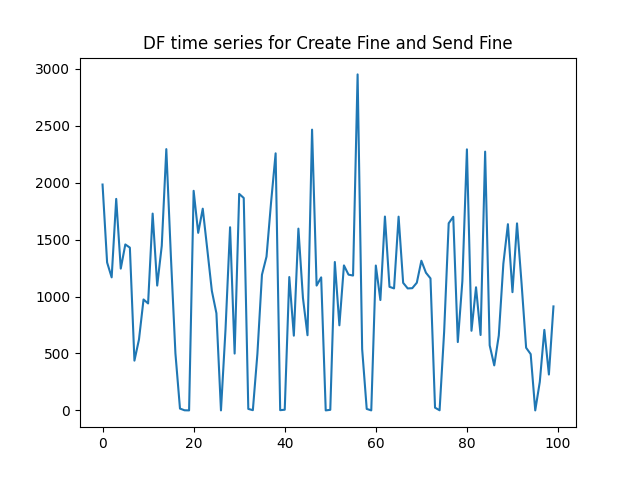
\includegraphics[width=0.49\textwidth]{./img/rtfmp_1.png}}
	\subfigure[50th most common DF - equisize]{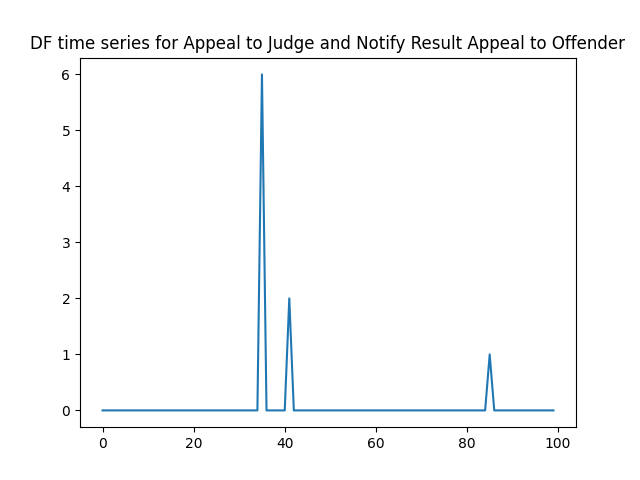
\includegraphics[width=0.49\textwidth]{./img/rtfmp_2.png}}
	\subfigure[Most common DF - equitemp]{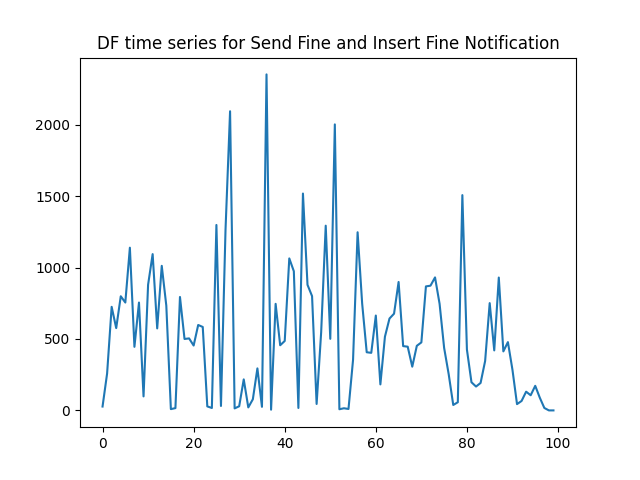
\includegraphics[width=0.49\textwidth]{./img/rtfmp_1_t.png}}
\subfigure[50th most common DF - equitemp]{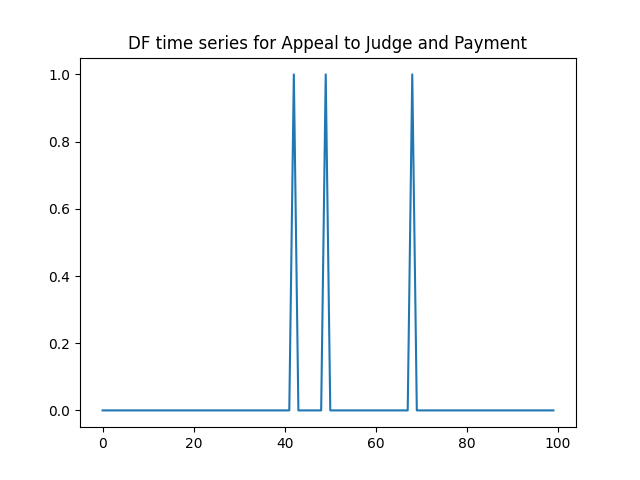
\includegraphics[width=0.49\textwidth]{./img/rtfmp_2_t.png}}
	\caption{RTFMP}
	\label{fig:rtfmpts}
\end{figure}

Resampling is based on a 10-fold cross-validation constructed following a rolling window approach for various horizon values $h\in[1,5]$ where a recursive strategy is used to iteratively obtain $\hat{y}_{t+h|T_{t+h-1}}$ with $(y_1,\dots,y_{T},\dots,\hat{y}_{t+h-1})$ \cite{weigend2018time}.
The 10 training sets exist from $(y_1,\dots,y_{T-h-f})$ and the test sets from\\ $(y_{T-h-f+1},\dots,y_{T-f})$ with $f\in[0,9]$ the fold index \cite{bergmeir2012use}.
While direct strategies with a separate model for every value of $h$ can be used as well and avoid the accumulation of error, they do not take into account statistical dependencies for subsequent predictions.

Given that we want to evaluate the capability of the approach to accurately predict the evolution of the process model, the combination of all DF predictions to obtain a global DFG prediction is considered.
The following two criteria are used:
\begin{itemize}
	\item Graph edit distance (GED) \cite{gao2010survey}: measures the similarity between two graphs based on the number of operations required to render the graphs isomorphic using edge and node insertions, deletion, or substitution.
	In this evaluation, it is used to check whether the forecasts are at least capable of returning similar structures by discerning whether a DF edge should exist between two activities regardless of how many directly follows relations occur.
	\item Cosine distance: measures the distance between two vectors and are often used to compare graph distance . This metric is used to compare the DFG's edge weight matrices between the actual and predicted number of DF relations.
\end{itemize}

\subsection{Results}
All pre-processing was done in Python with a combination of pm4py\footnote{\url{https://pm4py.fit.fraunhofer.de}} and the statsmodels package \cite{seabold2010statsmodels}. 
The code is available %TODOhere.

The cosine distance is reported in Tables \ref{tab:equisize_50} to \ref{tab:equitemp_100} where grayscale is used per event log to indicate the relative performance of each algorithm.
Generally, it can be found that naive forecasts are performing the worst overall, meaning that the DF time series forecasting does enjoy performance gains from a more intricate use of autocorrelations and/or decomposition.
Both decomposition techniques (SES and HW) perform similarly and adequately and consistently report the best result for each dataset for both interval and aggregation settings.
The same holds for simple AR models, where the lag-parameter $q$ occassionally offers slightly different results although this does not seem to be related with the number of intervals.
Results for ARIMA and GARCH models are mixed.
For ARIMA, the 3 best performing parameter sets are reported (with $q$ and $p$ used with values [1,4] and $d$ with values [0,1,2]).
They do not seem to be capable of outperforming simpeler AR models.
Overall, the simplest models seem to perform best and do not require extensive parameter tuning.
This might indicate that the time series do not exhibit intricate autocorrelations (ARIMA) and/or changing variance over time (GARCH). 

Finally, it can be noted that the cosine distance is slightly higher for longer horizon values, especially for the BPI 12 event log for which Figure \ref{fig:bpi12ts} showed stronger activity towards the end of the series still.
This phenomenom is typical of forecasting results as such predictions accumulate forecast errors.

% Table generated by Excel2LaTeX from sheet '50 intervals'
\begin{table}[htbp]
  \centering
    \begin{tabular}{|cl|rrrrrrrrrr|}
\cmidrule{3-12}    \multicolumn{1}{c}{} &       & \multicolumn{3}{c}{\textbf{AR}} & \multicolumn{3}{c}{\textbf{ARIMA}} &       &       &       &  \\
    \multicolumn{1}{r}{} & \textbf{h} & \multicolumn{1}{l}{\textbf{(1)}} & \multicolumn{1}{l}{\textbf{(2)}} & \multicolumn{1}{l}{\textbf{(4)}} & \multicolumn{1}{l}{\textbf{(2,1,1)}} & \multicolumn{1}{l}{\textbf{(2,1,2)}} & \multicolumn{1}{l}{\textbf{(4,1,1)}} & \multicolumn{1}{l}{\textbf{GARCH}} & \multicolumn{1}{l}{\textbf{HW}} & \multicolumn{1}{l}{\textbf{NAÏVE}} & \multicolumn{1}{l|}{\textbf{SES}} \\
    \midrule
    \multirow{5}[2]{*}{\textbf{RTFMP}} & \textbf{1} & \cellcolor[rgb]{ .847,  .847,  .847}1.873 & \cellcolor[rgb]{ .851,  .851,  .851}1.819 & \cellcolor[rgb]{ .843,  .843,  .843}1.892 & \cellcolor[rgb]{ .843,  .843,  .843}1.920 & \cellcolor[rgb]{ .839,  .839,  .839}1.956 & \cellcolor[rgb]{ .835,  .835,  .835}1.989 & \cellcolor[rgb]{ .784,  .784,  .784}2.553 & \cellcolor[rgb]{ .851,  .851,  .851}1.804 & \cellcolor[rgb]{ .757,  .757,  .757}2.821 & \cellcolor[rgb]{ .851,  .851,  .851}1.804 \\
          & \textbf{2} & \cellcolor[rgb]{ .831,  .831,  .831}2.047 & \cellcolor[rgb]{ .839,  .839,  .839}1.970 & \cellcolor[rgb]{ .831,  .831,  .831}2.028 & \cellcolor[rgb]{ .824,  .824,  .824}2.125 & \cellcolor[rgb]{ .82,  .82,  .82}2.141 & \cellcolor[rgb]{ .82,  .82,  .82}2.172 & \cellcolor[rgb]{ .686,  .686,  .686}3.590 & \cellcolor[rgb]{ .831,  .831,  .831}2.017 & \cellcolor[rgb]{ .741,  .741,  .741}2.998 & \cellcolor[rgb]{ .831,  .831,  .831}2.017 \\
          & \textbf{3} & \cellcolor[rgb]{ .839,  .839,  .839}1.965 & \cellcolor[rgb]{ .843,  .843,  .843}1.907 & \cellcolor[rgb]{ .843,  .843,  .843}1.928 & \cellcolor[rgb]{ .835,  .835,  .835}1.973 & \cellcolor[rgb]{ .835,  .835,  .835}1.998 & \cellcolor[rgb]{ .831,  .831,  .831}2.031 & \cellcolor[rgb]{ .675,  .675,  .675}3.705 & \cellcolor[rgb]{ .839,  .839,  .839}1.963 & \cellcolor[rgb]{ .733,  .733,  .733}3.082 & \cellcolor[rgb]{ .839,  .839,  .839}1.963 \\
          & \textbf{4} & \cellcolor[rgb]{ .835,  .835,  .835}2.005 & \cellcolor[rgb]{ .839,  .839,  .839}1.931 & \cellcolor[rgb]{ .839,  .839,  .839}1.957 & \cellcolor[rgb]{ .835,  .835,  .835}2.001 & \cellcolor[rgb]{ .831,  .831,  .831}2.017 & \cellcolor[rgb]{ .827,  .827,  .827}2.068 & \cellcolor[rgb]{ .667,  .667,  .667}3.807 & \cellcolor[rgb]{ .831,  .831,  .831}2.034 & \cellcolor[rgb]{ .749,  .749,  .749}2.896 & \cellcolor[rgb]{ .831,  .831,  .831}2.034 \\
          & \textbf{5} & \cellcolor[rgb]{ .827,  .827,  .827}2.060 & \cellcolor[rgb]{ .835,  .835,  .835}1.993 & \cellcolor[rgb]{ .835,  .835,  .835}1.986 & \cellcolor[rgb]{ .827,  .827,  .827}2.092 & \cellcolor[rgb]{ .827,  .827,  .827}2.081 & \cellcolor[rgb]{ .824,  .824,  .824}2.103 & \cellcolor[rgb]{ .651,  .651,  .651}3.946 & \cellcolor[rgb]{ .827,  .827,  .827}2.084 & \cellcolor[rgb]{ .761,  .761,  .761}2.775 & \cellcolor[rgb]{ .827,  .827,  .827}2.084 \\
    \midrule
    \multirow{5}[2]{*}{\textbf{BPI12}} & \textbf{1} & \cellcolor[rgb]{ .851,  .851,  .851}0.216 & \cellcolor[rgb]{ .851,  .851,  .851}0.212 & \cellcolor[rgb]{ .851,  .851,  .851}0.218 & \cellcolor[rgb]{ .843,  .843,  .843}0.242 & \cellcolor[rgb]{ .843,  .843,  .843}0.244 & \cellcolor[rgb]{ .843,  .843,  .843}0.244 & \cellcolor[rgb]{ .851,  .851,  .851}0.225 & \cellcolor[rgb]{ .847,  .847,  .847}0.235 & \cellcolor[rgb]{ .796,  .796,  .796}0.398 & \cellcolor[rgb]{ .847,  .847,  .847}0.235 \\
          & \textbf{2} & \cellcolor[rgb]{ .851,  .851,  .851}0.224 & \cellcolor[rgb]{ .847,  .847,  .847}0.229 & \cellcolor[rgb]{ .847,  .847,  .847}0.238 & \cellcolor[rgb]{ .835,  .835,  .835}0.273 & \cellcolor[rgb]{ .831,  .831,  .831}0.283 & \cellcolor[rgb]{ .835,  .835,  .835}0.268 & \cellcolor[rgb]{ .847,  .847,  .847}0.226 & \cellcolor[rgb]{ .843,  .843,  .843}0.243 & \cellcolor[rgb]{ .808,  .808,  .808}0.365 & \cellcolor[rgb]{ .843,  .843,  .843}0.243 \\
          & \textbf{3} & \cellcolor[rgb]{ .847,  .847,  .847}0.229 & \cellcolor[rgb]{ .847,  .847,  .847}0.228 & \cellcolor[rgb]{ .843,  .843,  .843}0.240 & \cellcolor[rgb]{ .831,  .831,  .831}0.281 & \cellcolor[rgb]{ .827,  .827,  .827}0.294 & \cellcolor[rgb]{ .831,  .831,  .831}0.284 & \cellcolor[rgb]{ .847,  .847,  .847}0.231 & \cellcolor[rgb]{ .843,  .843,  .843}0.248 & \cellcolor[rgb]{ .8,  .8,  .8}0.383 & \cellcolor[rgb]{ .843,  .843,  .843}0.248 \\
          & \textbf{4} & \cellcolor[rgb]{ .792,  .792,  .792}0.416 & \cellcolor[rgb]{ .792,  .792,  .792}0.410 & \cellcolor[rgb]{ .788,  .788,  .788}0.423 & \cellcolor[rgb]{ .773,  .773,  .773}0.481 & \cellcolor[rgb]{ .773,  .773,  .773}0.474 & \cellcolor[rgb]{ .776,  .776,  .776}0.466 & \cellcolor[rgb]{ .792,  .792,  .792}0.416 & \cellcolor[rgb]{ .784,  .784,  .784}0.437 & \cellcolor[rgb]{ .733,  .733,  .733}0.608 & \cellcolor[rgb]{ .784,  .784,  .784}0.437 \\
          & \textbf{5} & \cellcolor[rgb]{ .706,  .706,  .706}0.697 & \cellcolor[rgb]{ .71,  .71,  .71}0.681 & \cellcolor[rgb]{ .71,  .71,  .71}0.690 & \cellcolor[rgb]{ .694,  .694,  .694}0.737 & \cellcolor[rgb]{ .702,  .702,  .702}0.715 & \cellcolor[rgb]{ .706,  .706,  .706}0.703 & \cellcolor[rgb]{ .706,  .706,  .706}0.693 & \cellcolor[rgb]{ .706,  .706,  .706}0.691 & \cellcolor[rgb]{ .651,  .651,  .651}0.871 & \cellcolor[rgb]{ .706,  .706,  .706}0.691 \\
    \midrule
    \multirow{5}[2]{*}{\textbf{Sepsis}} & \textbf{1} & \cellcolor[rgb]{ .839,  .839,  .839}0.996 & \cellcolor[rgb]{ .831,  .831,  .831}1.023 & \cellcolor[rgb]{ .824,  .824,  .824}1.060 & \cellcolor[rgb]{ .816,  .816,  .816}1.088 & \cellcolor[rgb]{ .816,  .816,  .816}1.093 & \cellcolor[rgb]{ .812,  .812,  .812}1.107 & \cellcolor[rgb]{ .843,  .843,  .843}0.980 & \cellcolor[rgb]{ .843,  .843,  .843}0.981 & \cellcolor[rgb]{ .663,  .663,  .663}1.727 & \cellcolor[rgb]{ .843,  .843,  .843}0.981 \\
          & \textbf{2} & \cellcolor[rgb]{ .851,  .851,  .851}0.940 & \cellcolor[rgb]{ .847,  .847,  .847}0.965 & \cellcolor[rgb]{ .835,  .835,  .835}1.003 & \cellcolor[rgb]{ .827,  .827,  .827}1.039 & \cellcolor[rgb]{ .835,  .835,  .835}1.005 & \cellcolor[rgb]{ .831,  .831,  .831}1.030 & \cellcolor[rgb]{ .851,  .851,  .851}0.946 & \cellcolor[rgb]{ .847,  .847,  .847}0.955 & \cellcolor[rgb]{ .659,  .659,  .659}1.743 & \cellcolor[rgb]{ .847,  .847,  .847}0.955 \\
          & \textbf{3} & \cellcolor[rgb]{ .843,  .843,  .843}0.967 & \cellcolor[rgb]{ .843,  .843,  .843}0.975 & \cellcolor[rgb]{ .839,  .839,  .839}0.990 & \cellcolor[rgb]{ .824,  .824,  .824}1.055 & \cellcolor[rgb]{ .831,  .831,  .831}1.018 & \cellcolor[rgb]{ .827,  .827,  .827}1.037 & \cellcolor[rgb]{ .843,  .843,  .843}0.974 & \cellcolor[rgb]{ .843,  .843,  .843}0.973 & \cellcolor[rgb]{ .651,  .651,  .651}1.775 & \cellcolor[rgb]{ .843,  .843,  .843}0.973 \\
          & \textbf{4} & \cellcolor[rgb]{ .851,  .851,  .851}0.938 & \cellcolor[rgb]{ .851,  .851,  .851}0.940 & \cellcolor[rgb]{ .847,  .847,  .847}0.949 & \cellcolor[rgb]{ .831,  .831,  .831}1.023 & \cellcolor[rgb]{ .839,  .839,  .839}0.995 & \cellcolor[rgb]{ .827,  .827,  .827}1.040 & \cellcolor[rgb]{ .851,  .851,  .851}0.940 & \cellcolor[rgb]{ .851,  .851,  .851}0.943 & \cellcolor[rgb]{ .667,  .667,  .667}1.719 & \cellcolor[rgb]{ .851,  .851,  .851}0.943 \\
          & \textbf{5} & \cellcolor[rgb]{ .851,  .851,  .851}0.936 & \cellcolor[rgb]{ .851,  .851,  .851}0.937 & \cellcolor[rgb]{ .847,  .847,  .847}0.952 & \cellcolor[rgb]{ .839,  .839,  .839}0.996 & \cellcolor[rgb]{ .843,  .843,  .843}0.976 & \cellcolor[rgb]{ .839,  .839,  .839}0.996 & \cellcolor[rgb]{ .851,  .851,  .851}0.932 & \cellcolor[rgb]{ .851,  .851,  .851}0.939 & \cellcolor[rgb]{ .702,  .702,  .702}1.564 & \cellcolor[rgb]{ .851,  .851,  .851}0.939 \\
    \bottomrule
    \end{tabular}%
  \caption{Cosine distance results for $h=5$ and 50 intervals with equisized aggregation.}
  \label{tab:equisize_50}%
\end{table}%

% Table generated by Excel2LaTeX from sheet '50 intervals'
\begin{table}[htbp]
  \centering
  \resizebox{0.7\textwidth}{!}{
    \begin{tabular}{|cl|rrrrrrrrrr|}
\cmidrule{3-12}    \multicolumn{1}{c}{} &       & \multicolumn{3}{c}{\textbf{AR}} & \multicolumn{3}{c}{\textbf{ARIMA}} &       &       &       &  \\
    \multicolumn{1}{r}{} & \textbf{h} & \multicolumn{1}{l}{\textbf{(1)}} & \multicolumn{1}{l}{\textbf{(2)}} & \multicolumn{1}{l}{\textbf{(4)}} & \multicolumn{1}{l}{\textbf{(2,1,1)}} & \multicolumn{1}{l}{\textbf{(2,1,2)}} & \multicolumn{1}{l}{\textbf{(4,1,1)}} & \multicolumn{1}{l}{\textbf{GARCH}} & \multicolumn{1}{l}{\textbf{HW}} & \multicolumn{1}{l}{\textbf{NAÏVE}} & \multicolumn{1}{l|}{\textbf{SES}} \\
    \midrule
    \multirow{5}[2]{*}{\textbf{RTFMP}} & \textbf{1} & \cellcolor[rgb]{ .839,  .839,  .839}2.232 & \cellcolor[rgb]{ .847,  .847,  .847}2.177 & \cellcolor[rgb]{ .851,  .851,  .851}2.105 & \cellcolor[rgb]{ .831,  .831,  .831}2.334 & \cellcolor[rgb]{ .831,  .831,  .831}2.318 & \cellcolor[rgb]{ .835,  .835,  .835}2.288 & \cellcolor[rgb]{ .808,  .808,  .808}2.602 & \cellcolor[rgb]{ .816,  .816,  .816}2.515 & \cellcolor[rgb]{ .796,  .796,  .796}2.721 & \cellcolor[rgb]{ .816,  .816,  .816}2.515 \\
          & \textbf{2} & \cellcolor[rgb]{ .82,  .82,  .82}2.459 & \cellcolor[rgb]{ .824,  .824,  .824}2.426 & \cellcolor[rgb]{ .831,  .831,  .831}2.352 & \cellcolor[rgb]{ .812,  .812,  .812}2.554 & \cellcolor[rgb]{ .812,  .812,  .812}2.532 & \cellcolor[rgb]{ .816,  .816,  .816}2.499 & \cellcolor[rgb]{ .816,  .816,  .816}2.499 & \cellcolor[rgb]{ .82,  .82,  .82}2.459 & \cellcolor[rgb]{ .69,  .69,  .69}3.807 & \cellcolor[rgb]{ .82,  .82,  .82}2.459 \\
          & \textbf{3} & \cellcolor[rgb]{ .812,  .812,  .812}2.540 & \cellcolor[rgb]{ .816,  .816,  .816}2.489 & \cellcolor[rgb]{ .824,  .824,  .824}2.426 & \cellcolor[rgb]{ .804,  .804,  .804}2.608 & \cellcolor[rgb]{ .808,  .808,  .808}2.586 & \cellcolor[rgb]{ .808,  .808,  .808}2.577 & \cellcolor[rgb]{ .812,  .812,  .812}2.540 & \cellcolor[rgb]{ .812,  .812,  .812}2.535 & \cellcolor[rgb]{ .659,  .659,  .659}4.175 & \cellcolor[rgb]{ .812,  .812,  .812}2.535 \\
          & \textbf{4} & \cellcolor[rgb]{ .816,  .816,  .816}2.497 & \cellcolor[rgb]{ .816,  .816,  .816}2.488 & \cellcolor[rgb]{ .82,  .82,  .82}2.438 & \cellcolor[rgb]{ .812,  .812,  .812}2.533 & \cellcolor[rgb]{ .816,  .816,  .816}2.515 & \cellcolor[rgb]{ .812,  .812,  .812}2.553 & \cellcolor[rgb]{ .816,  .816,  .816}2.518 & \cellcolor[rgb]{ .82,  .82,  .82}2.464 & \cellcolor[rgb]{ .655,  .655,  .655}4.188 & \cellcolor[rgb]{ .82,  .82,  .82}2.464 \\
          & \textbf{5} & \cellcolor[rgb]{ .8,  .8,  .8}2.685 & \cellcolor[rgb]{ .796,  .796,  .796}2.693 & \cellcolor[rgb]{ .8,  .8,  .8}2.655 & \cellcolor[rgb]{ .796,  .796,  .796}2.724 & \cellcolor[rgb]{ .796,  .796,  .796}2.722 & \cellcolor[rgb]{ .796,  .796,  .796}2.723 & \cellcolor[rgb]{ .792,  .792,  .792}2.743 & \cellcolor[rgb]{ .8,  .8,  .8}2.651 & \cellcolor[rgb]{ .651,  .651,  .651}4.222 & \cellcolor[rgb]{ .8,  .8,  .8}2.651 \\
\cmidrule{1-2}    \multirow{5}[2]{*}{\textbf{BPI12}} & \textbf{1} & \cellcolor[rgb]{ .851,  .851,  .851}0.427 & \cellcolor[rgb]{ .851,  .851,  .851}0.429 & \cellcolor[rgb]{ .851,  .851,  .851}0.435 & \cellcolor[rgb]{ .847,  .847,  .847}0.457 & \cellcolor[rgb]{ .847,  .847,  .847}0.464 & \cellcolor[rgb]{ .847,  .847,  .847}0.459 & \cellcolor[rgb]{ .851,  .851,  .851}0.420 & \cellcolor[rgb]{ .847,  .847,  .847}0.447 & \cellcolor[rgb]{ .816,  .816,  .816}0.626 & \cellcolor[rgb]{ .847,  .847,  .847}0.447 \\
          & \textbf{2} & \cellcolor[rgb]{ .839,  .839,  .839}0.504 & \cellcolor[rgb]{ .839,  .839,  .839}0.503 & \cellcolor[rgb]{ .839,  .839,  .839}0.504 & \cellcolor[rgb]{ .835,  .835,  .835}0.533 & \cellcolor[rgb]{ .831,  .831,  .831}0.538 & \cellcolor[rgb]{ .831,  .831,  .831}0.535 & \cellcolor[rgb]{ .839,  .839,  .839}0.496 & \cellcolor[rgb]{ .835,  .835,  .835}0.527 & \cellcolor[rgb]{ .78,  .78,  .78}0.837 & \cellcolor[rgb]{ .835,  .835,  .835}0.527 \\
          & \textbf{3} & \cellcolor[rgb]{ .792,  .792,  .792}0.768 & \cellcolor[rgb]{ .792,  .792,  .792}0.763 & \cellcolor[rgb]{ .792,  .792,  .792}0.762 & \cellcolor[rgb]{ .788,  .788,  .788}0.795 & \cellcolor[rgb]{ .788,  .788,  .788}0.799 & \cellcolor[rgb]{ .784,  .784,  .784}0.811 & \cellcolor[rgb]{ .792,  .792,  .792}0.763 & \cellcolor[rgb]{ .788,  .788,  .788}0.794 & \cellcolor[rgb]{ .753,  .753,  .753}1.008 & \cellcolor[rgb]{ .788,  .788,  .788}0.794 \\
          & \textbf{4} & \cellcolor[rgb]{ .749,  .749,  .749}1.025 & \cellcolor[rgb]{ .749,  .749,  .749}1.017 & \cellcolor[rgb]{ .753,  .753,  .753}1.011 & \cellcolor[rgb]{ .745,  .745,  .745}1.055 & \cellcolor[rgb]{ .741,  .741,  .741}1.067 & \cellcolor[rgb]{ .737,  .737,  .737}1.094 & \cellcolor[rgb]{ .749,  .749,  .749}1.016 & \cellcolor[rgb]{ .745,  .745,  .745}1.056 & \cellcolor[rgb]{ .682,  .682,  .682}1.401 & \cellcolor[rgb]{ .745,  .745,  .745}1.056 \\
          & \textbf{5} & \cellcolor[rgb]{ .702,  .702,  .702}1.304 & \cellcolor[rgb]{ .702,  .702,  .702}1.288 & \cellcolor[rgb]{ .706,  .706,  .706}1.264 & \cellcolor[rgb]{ .702,  .702,  .702}1.287 & \cellcolor[rgb]{ .702,  .702,  .702}1.300 & \cellcolor[rgb]{ .694,  .694,  .694}1.350 & \cellcolor[rgb]{ .702,  .702,  .702}1.291 & \cellcolor[rgb]{ .702,  .702,  .702}1.297 & \cellcolor[rgb]{ .651,  .651,  .651}1.582 & \cellcolor[rgb]{ .702,  .702,  .702}1.297 \\
\cmidrule{1-2}    \multirow{5}[2]{*}{\textbf{Sepsis}} & \textbf{1} & \cellcolor[rgb]{ .851,  .851,  .851}1.169 & \cellcolor[rgb]{ .851,  .851,  .851}1.176 & \cellcolor[rgb]{ .847,  .847,  .847}1.201 & \cellcolor[rgb]{ .843,  .843,  .843}1.220 & \cellcolor[rgb]{ .843,  .843,  .843}1.211 & \cellcolor[rgb]{ .835,  .835,  .835}1.247 & \cellcolor[rgb]{ .847,  .847,  .847}1.185 & \cellcolor[rgb]{ .851,  .851,  .851}1.173 & \cellcolor[rgb]{ .714,  .714,  .714}1.880 & \cellcolor[rgb]{ .851,  .851,  .851}1.173 \\
          & \textbf{2} & \cellcolor[rgb]{ .851,  .851,  .851}1.169 & \cellcolor[rgb]{ .851,  .851,  .851}1.175 & \cellcolor[rgb]{ .843,  .843,  .843}1.214 & \cellcolor[rgb]{ .839,  .839,  .839}1.228 & \cellcolor[rgb]{ .839,  .839,  .839}1.237 & \cellcolor[rgb]{ .831,  .831,  .831}1.267 & \cellcolor[rgb]{ .851,  .851,  .851}1.171 & \cellcolor[rgb]{ .851,  .851,  .851}1.169 & \cellcolor[rgb]{ .663,  .663,  .663}2.134 & \cellcolor[rgb]{ .851,  .851,  .851}1.169 \\
          & \textbf{3} & \cellcolor[rgb]{ .851,  .851,  .851}1.165 & \cellcolor[rgb]{ .851,  .851,  .851}1.162 & \cellcolor[rgb]{ .843,  .843,  .843}1.203 & \cellcolor[rgb]{ .839,  .839,  .839}1.227 & \cellcolor[rgb]{ .839,  .839,  .839}1.232 & \cellcolor[rgb]{ .831,  .831,  .831}1.269 & \cellcolor[rgb]{ .851,  .851,  .851}1.172 & \cellcolor[rgb]{ .851,  .851,  .851}1.176 & \cellcolor[rgb]{ .651,  .651,  .651}2.185 & \cellcolor[rgb]{ .851,  .851,  .851}1.176 \\
          & \textbf{4} & \cellcolor[rgb]{ .851,  .851,  .851}1.177 & \cellcolor[rgb]{ .851,  .851,  .851}1.179 & \cellcolor[rgb]{ .843,  .843,  .843}1.216 & \cellcolor[rgb]{ .843,  .843,  .843}1.220 & \cellcolor[rgb]{ .835,  .835,  .835}1.249 & \cellcolor[rgb]{ .831,  .831,  .831}1.271 & \cellcolor[rgb]{ .847,  .847,  .847}1.185 & \cellcolor[rgb]{ .851,  .851,  .851}1.177 & \cellcolor[rgb]{ .667,  .667,  .667}2.108 & \cellcolor[rgb]{ .851,  .851,  .851}1.177 \\
          & \textbf{5} & \cellcolor[rgb]{ .843,  .843,  .843}1.205 & \cellcolor[rgb]{ .843,  .843,  .843}1.203 & \cellcolor[rgb]{ .843,  .843,  .843}1.212 & \cellcolor[rgb]{ .835,  .835,  .835}1.248 & \cellcolor[rgb]{ .835,  .835,  .835}1.257 & \cellcolor[rgb]{ .835,  .835,  .835}1.249 & \cellcolor[rgb]{ .843,  .843,  .843}1.214 & \cellcolor[rgb]{ .843,  .843,  .843}1.213 & \cellcolor[rgb]{ .655,  .655,  .655}2.178 & \cellcolor[rgb]{ .843,  .843,  .843}1.213 \\
    \bottomrule
    \end{tabular}
    }
  \caption{Cosine distance results for $h=5$ and 100 intervals with equisized aggregation.}
  \label{tab:equisize_100}%
\end{table}%

\begin{table}[htbp]
  \centering
    \begin{tabular}{|cl|rrrrrrrrrr|}
\cmidrule{3-12}    \multicolumn{1}{r}{} &       & \multicolumn{3}{c}{\textbf{AR}} & \multicolumn{3}{c}{\textbf{ARIMA}} &       &       &       &  \\
    \multicolumn{1}{r}{} & \textbf{h} & \multicolumn{1}{c}{\textbf{(1)}} & \multicolumn{1}{c}{\textbf{(2)}} & \multicolumn{1}{c}{\textbf{(4)}} & \multicolumn{1}{c}{\textbf{(2,1,1)}} & \multicolumn{1}{c}{\textbf{(2,1,2)}} & \multicolumn{1}{c}{\textbf{(4,1,1)}} & \multicolumn{1}{c}{\textbf{GARCH}} & \multicolumn{1}{c}{\textbf{HW}} & \multicolumn{1}{c}{\textbf{NAÏVE}} & \multicolumn{1}{c|}{\textbf{SES}} \\
    \midrule
    \multirow{5}[2]{*}{\textbf{RTFMP}} & \textbf{1} & \cellcolor[rgb]{ .843,  .843,  .843}1.884 & \cellcolor[rgb]{ .839,  .839,  .839}1.917 & \cellcolor[rgb]{ .847,  .847,  .847}1.877 & \cellcolor[rgb]{ .843,  .843,  .843}1.896 & \cellcolor[rgb]{ .835,  .835,  .835}1.965 & \cellcolor[rgb]{ .835,  .835,  .835}1.966 & \cellcolor[rgb]{ .827,  .827,  .827}2.011 & \cellcolor[rgb]{ .843,  .843,  .843}1.898 & \cellcolor[rgb]{ .773,  .773,  .773}2.494 & \cellcolor[rgb]{ .843,  .843,  .843}1.898 \\
          & \textbf{2} & \cellcolor[rgb]{ .847,  .847,  .847}1.864 & \cellcolor[rgb]{ .847,  .847,  .847}1.877 & \cellcolor[rgb]{ .851,  .851,  .851}1.815 & \cellcolor[rgb]{ .847,  .847,  .847}1.871 & \cellcolor[rgb]{ .843,  .843,  .843}1.903 & \cellcolor[rgb]{ .835,  .835,  .835}1.970 & \cellcolor[rgb]{ .843,  .843,  .843}1.892 & \cellcolor[rgb]{ .847,  .847,  .847}1.857 & \cellcolor[rgb]{ .675,  .675,  .675}3.276 & \cellcolor[rgb]{ .847,  .847,  .847}1.857 \\
          & \textbf{3} & \cellcolor[rgb]{ .843,  .843,  .843}1.904 & \cellcolor[rgb]{ .843,  .843,  .843}1.881 & \cellcolor[rgb]{ .851,  .851,  .851}1.815 & \cellcolor[rgb]{ .847,  .847,  .847}1.874 & \cellcolor[rgb]{ .847,  .847,  .847}1.865 & \cellcolor[rgb]{ .827,  .827,  .827}2.025 & \cellcolor[rgb]{ .839,  .839,  .839}1.937 & \cellcolor[rgb]{ .843,  .843,  .843}1.888 & \cellcolor[rgb]{ .714,  .714,  .714}2.953 & \cellcolor[rgb]{ .843,  .843,  .843}1.888 \\
          & \textbf{4} & \cellcolor[rgb]{ .827,  .827,  .827}2.026 & \cellcolor[rgb]{ .831,  .831,  .831}1.999 & \cellcolor[rgb]{ .851,  .851,  .851}1.841 & \cellcolor[rgb]{ .831,  .831,  .831}1.980 & \cellcolor[rgb]{ .839,  .839,  .839}1.923 & \cellcolor[rgb]{ .824,  .824,  .824}2.072 & \cellcolor[rgb]{ .827,  .827,  .827}2.039 & \cellcolor[rgb]{ .831,  .831,  .831}1.996 & \cellcolor[rgb]{ .741,  .741,  .741}2.738 & \cellcolor[rgb]{ .831,  .831,  .831}1.996 \\
          & \textbf{5} & \cellcolor[rgb]{ .8,  .8,  .8}2.239 & \cellcolor[rgb]{ .804,  .804,  .804}2.214 & \cellcolor[rgb]{ .808,  .808,  .808}2.175 & \cellcolor[rgb]{ .804,  .804,  .804}2.229 & \cellcolor[rgb]{ .8,  .8,  .8}2.246 & \cellcolor[rgb]{ .784,  .784,  .784}2.398 & \cellcolor[rgb]{ .804,  .804,  .804}2.219 & \cellcolor[rgb]{ .796,  .796,  .796}2.278 & \cellcolor[rgb]{ .651,  .651,  .651}3.469 & \cellcolor[rgb]{ .796,  .796,  .796}2.278 \\
    \midrule
    \multirow{5}[2]{*}{\textbf{BPI12}} & \textbf{1} & \cellcolor[rgb]{ .847,  .847,  .847}0.313 & \cellcolor[rgb]{ .851,  .851,  .851}0.280 & \cellcolor[rgb]{ .851,  .851,  .851}0.277 & \cellcolor[rgb]{ .847,  .847,  .847}0.309 & \cellcolor[rgb]{ .847,  .847,  .847}0.304 & \cellcolor[rgb]{ .847,  .847,  .847}0.304 & \cellcolor[rgb]{ .851,  .851,  .851}0.291 & \cellcolor[rgb]{ .843,  .843,  .843}0.332 & \cellcolor[rgb]{ .808,  .808,  .808}0.561 & \cellcolor[rgb]{ .843,  .843,  .843}0.332 \\
          & \textbf{2} & \cellcolor[rgb]{ .831,  .831,  .831}0.398 & \cellcolor[rgb]{ .831,  .831,  .831}0.402 & \cellcolor[rgb]{ .831,  .831,  .831}0.402 & \cellcolor[rgb]{ .831,  .831,  .831}0.411 & \cellcolor[rgb]{ .831,  .831,  .831}0.414 & \cellcolor[rgb]{ .827,  .827,  .827}0.422 & \cellcolor[rgb]{ .831,  .831,  .831}0.402 & \cellcolor[rgb]{ .831,  .831,  .831}0.402 & \cellcolor[rgb]{ .82,  .82,  .82}0.467 & \cellcolor[rgb]{ .831,  .831,  .831}0.402 \\
          & \textbf{3} & \cellcolor[rgb]{ .784,  .784,  .784}0.688 & \cellcolor[rgb]{ .792,  .792,  .792}0.634 & \cellcolor[rgb]{ .792,  .792,  .792}0.645 & \cellcolor[rgb]{ .788,  .788,  .788}0.674 & \cellcolor[rgb]{ .788,  .788,  .788}0.672 & \cellcolor[rgb]{ .784,  .784,  .784}0.693 & \cellcolor[rgb]{ .788,  .788,  .788}0.678 & \cellcolor[rgb]{ .784,  .784,  .784}0.682 & \cellcolor[rgb]{ .729,  .729,  .729}1.032 & \cellcolor[rgb]{ .784,  .784,  .784}0.682 \\
          & \textbf{4} & \cellcolor[rgb]{ .741,  .741,  .741}0.949 & \cellcolor[rgb]{ .749,  .749,  .749}0.901 & \cellcolor[rgb]{ .749,  .749,  .749}0.904 & \cellcolor[rgb]{ .753,  .753,  .753}0.891 & \cellcolor[rgb]{ .749,  .749,  .749}0.905 & \cellcolor[rgb]{ .749,  .749,  .749}0.901 & \cellcolor[rgb]{ .745,  .745,  .745}0.920 & \cellcolor[rgb]{ .757,  .757,  .757}0.857 & \cellcolor[rgb]{ .741,  .741,  .741}0.952 & \cellcolor[rgb]{ .757,  .757,  .757}0.857 \\
          & \textbf{5} & \cellcolor[rgb]{ .698,  .698,  .698}1.212 & \cellcolor[rgb]{ .718,  .718,  .718}1.091 & \cellcolor[rgb]{ .718,  .718,  .718}1.095 & \cellcolor[rgb]{ .718,  .718,  .718}1.097 & \cellcolor[rgb]{ .714,  .714,  .714}1.110 & \cellcolor[rgb]{ .718,  .718,  .718}1.094 & \cellcolor[rgb]{ .706,  .706,  .706}1.177 & \cellcolor[rgb]{ .718,  .718,  .718}1.102 & \cellcolor[rgb]{ .651,  .651,  .651}1.488 & \cellcolor[rgb]{ .718,  .718,  .718}1.102 \\
    \midrule
    \multirow{5}[2]{*}{\textbf{Sepsis}} & \textbf{1} & \cellcolor[rgb]{ .78,  .78,  .78}0.887 & \cellcolor[rgb]{ .753,  .753,  .753}1.020 & \cellcolor[rgb]{ .737,  .737,  .737}1.102 & \cellcolor[rgb]{ .714,  .714,  .714}1.206 & \cellcolor[rgb]{ .682,  .682,  .682}1.362 & \cellcolor[rgb]{ .686,  .686,  .686}1.358 & \cellcolor[rgb]{ .776,  .776,  .776}0.899 & \cellcolor[rgb]{ .737,  .737,  .737}1.091 & \cellcolor[rgb]{ .655,  .655,  .655}1.508 & \cellcolor[rgb]{ .737,  .737,  .737}1.091 \\
          & \textbf{2} & \cellcolor[rgb]{ .812,  .812,  .812}0.727 & \cellcolor[rgb]{ .792,  .792,  .792}0.832 & \cellcolor[rgb]{ .776,  .776,  .776}0.911 & \cellcolor[rgb]{ .741,  .741,  .741}1.070 & \cellcolor[rgb]{ .714,  .714,  .714}1.219 & \cellcolor[rgb]{ .718,  .718,  .718}1.201 & \cellcolor[rgb]{ .804,  .804,  .804}0.771 & \cellcolor[rgb]{ .776,  .776,  .776}0.909 & \cellcolor[rgb]{ .651,  .651,  .651}1.514 & \cellcolor[rgb]{ .776,  .776,  .776}0.909 \\
          & \textbf{3} & \cellcolor[rgb]{ .831,  .831,  .831}0.637 & \cellcolor[rgb]{ .824,  .824,  .824}0.665 & \cellcolor[rgb]{ .812,  .812,  .812}0.732 & \cellcolor[rgb]{ .776,  .776,  .776}0.907 & \cellcolor[rgb]{ .722,  .722,  .722}1.168 & \cellcolor[rgb]{ .753,  .753,  .753}1.022 & \cellcolor[rgb]{ .82,  .82,  .82}0.681 & \cellcolor[rgb]{ .8,  .8,  .8}0.787 & \cellcolor[rgb]{ .671,  .671,  .671}1.421 & \cellcolor[rgb]{ .8,  .8,  .8}0.787 \\
          & \textbf{4} & \cellcolor[rgb]{ .839,  .839,  .839}0.598 & \cellcolor[rgb]{ .839,  .839,  .839}0.601 & \cellcolor[rgb]{ .827,  .827,  .827}0.659 & \cellcolor[rgb]{ .784,  .784,  .784}0.871 & \cellcolor[rgb]{ .745,  .745,  .745}1.064 & \cellcolor[rgb]{ .769,  .769,  .769}0.947 & \cellcolor[rgb]{ .831,  .831,  .831}0.639 & \cellcolor[rgb]{ .816,  .816,  .816}0.720 & \cellcolor[rgb]{ .663,  .663,  .663}1.464 & \cellcolor[rgb]{ .816,  .816,  .816}0.720 \\
          & \textbf{5} & \cellcolor[rgb]{ .851,  .851,  .851}0.541 & \cellcolor[rgb]{ .851,  .851,  .851}0.526 & \cellcolor[rgb]{ .843,  .843,  .843}0.570 & \cellcolor[rgb]{ .804,  .804,  .804}0.777 & \cellcolor[rgb]{ .753,  .753,  .753}1.017 & \cellcolor[rgb]{ .784,  .784,  .784}0.862 & \cellcolor[rgb]{ .843,  .843,  .843}0.580 & \cellcolor[rgb]{ .831,  .831,  .831}0.636 & \cellcolor[rgb]{ .71,  .71,  .71}1.232 & \cellcolor[rgb]{ .831,  .831,  .831}0.636 \\
    \bottomrule
    \end{tabular}%
  \caption{Cosine distance results for $h=5$ and 50 intervals with equitemporal aggregation.}
  \label{tab:equitemp_50}%
\end{table}%

% Table generated by Excel2LaTeX from sheet 'equitemp'
\begin{table}[htbp]
  \centering
  \resizebox{0.7\textwidth}{!}{
    \begin{tabular}{|cl|rrrrrrrrrr|}
\cmidrule{3-12}    \multicolumn{1}{r}{} &       & \multicolumn{3}{c}{\textbf{AR}} & \multicolumn{3}{c}{\textbf{ARIMA}} &       &       &       &  \\
    \multicolumn{1}{r}{} & \textbf{h} & \multicolumn{1}{c}{\textbf{(1)}} & \multicolumn{1}{c}{\textbf{(2)}} & \multicolumn{1}{c}{\textbf{(4)}} & \multicolumn{1}{c}{\textbf{(2,1,1)}} & \multicolumn{1}{c}{\textbf{(2,1,2)}} & \multicolumn{1}{c}{\textbf{(4,1,1)}} & \multicolumn{1}{c}{\textbf{GARCH}} & \multicolumn{1}{c}{\textbf{HW}} & \multicolumn{1}{c}{\textbf{NAÏVE}} & \multicolumn{1}{c|}{\textbf{SES}} \\
    \midrule
    \multirow{5}[2]{*}{\textbf{RTFMP}} & \textbf{1} & \cellcolor[rgb]{ .824,  .824,  .824}1.833 & \cellcolor[rgb]{ .824,  .824,  .824}1.814 & \cellcolor[rgb]{ .808,  .808,  .808}1.969 & \cellcolor[rgb]{ .812,  .812,  .812}1.927 & \cellcolor[rgb]{ .812,  .812,  .812}1.945 & \cellcolor[rgb]{ .796,  .796,  .796}2.062 & \cellcolor[rgb]{ .82,  .82,  .82}1.863 & \cellcolor[rgb]{ .827,  .827,  .827}1.801 & \cellcolor[rgb]{ .749,  .749,  .749}2.457 & \cellcolor[rgb]{ .827,  .827,  .827}1.801 \\
          & \textbf{2} & \cellcolor[rgb]{ .816,  .816,  .816}1.893 & \cellcolor[rgb]{ .827,  .827,  .827}1.806 & \cellcolor[rgb]{ .82,  .82,  .82}1.879 & \cellcolor[rgb]{ .82,  .82,  .82}1.855 & \cellcolor[rgb]{ .835,  .835,  .835}1.718 & \cellcolor[rgb]{ .82,  .82,  .82}1.879 & \cellcolor[rgb]{ .824,  .824,  .824}1.822 & \cellcolor[rgb]{ .808,  .808,  .808}1.965 & \cellcolor[rgb]{ .706,  .706,  .706}2.855 & \cellcolor[rgb]{ .808,  .808,  .808}1.965 \\
          & \textbf{3} & \cellcolor[rgb]{ .824,  .824,  .824}1.844 & \cellcolor[rgb]{ .827,  .827,  .827}1.782 & \cellcolor[rgb]{ .824,  .824,  .824}1.823 & \cellcolor[rgb]{ .827,  .827,  .827}1.799 & \cellcolor[rgb]{ .851,  .851,  .851}1.601 & \cellcolor[rgb]{ .824,  .824,  .824}1.828 & \cellcolor[rgb]{ .831,  .831,  .831}1.778 & \cellcolor[rgb]{ .8,  .8,  .8}2.049 & \cellcolor[rgb]{ .651,  .651,  .651}3.305 & \cellcolor[rgb]{ .8,  .8,  .8}2.049 \\
          & \textbf{4} & \cellcolor[rgb]{ .82,  .82,  .82}1.848 & \cellcolor[rgb]{ .827,  .827,  .827}1.803 & \cellcolor[rgb]{ .827,  .827,  .827}1.802 & \cellcolor[rgb]{ .82,  .82,  .82}1.847 & \cellcolor[rgb]{ .851,  .851,  .851}1.574 & \cellcolor[rgb]{ .831,  .831,  .831}1.759 & \cellcolor[rgb]{ .827,  .827,  .827}1.806 & \cellcolor[rgb]{ .792,  .792,  .792}2.093 & \cellcolor[rgb]{ .663,  .663,  .663}3.229 & \cellcolor[rgb]{ .792,  .792,  .792}2.093 \\
          & \textbf{5} & \cellcolor[rgb]{ .796,  .796,  .796}2.057 & \cellcolor[rgb]{ .8,  .8,  .8}2.031 & \cellcolor[rgb]{ .8,  .8,  .8}2.016 & \cellcolor[rgb]{ .796,  .796,  .796}2.051 & \cellcolor[rgb]{ .82,  .82,  .82}1.855 & \cellcolor[rgb]{ .804,  .804,  .804}2.015 & \cellcolor[rgb]{ .8,  .8,  .8}2.042 & \cellcolor[rgb]{ .776,  .776,  .776}2.244 & \cellcolor[rgb]{ .659,  .659,  .659}3.254 & \cellcolor[rgb]{ .776,  .776,  .776}2.244 \\
\cmidrule{1-2}    \multirow{5}[2]{*}{\textbf{BPI12}} & \textbf{1} & \cellcolor[rgb]{ .839,  .839,  .839}1.179 & \cellcolor[rgb]{ .816,  .816,  .816}1.275 & \cellcolor[rgb]{ .843,  .843,  .843}1.155 & \cellcolor[rgb]{ .835,  .835,  .835}1.190 & \cellcolor[rgb]{ .827,  .827,  .827}1.235 & \cellcolor[rgb]{ .851,  .851,  .851}1.133 & \cellcolor[rgb]{ .839,  .839,  .839}1.182 & \cellcolor[rgb]{ .851,  .851,  .851}1.118 & \cellcolor[rgb]{ .816,  .816,  .816}1.282 & \cellcolor[rgb]{ .851,  .851,  .851}1.118 \\
          & \textbf{2} & \cellcolor[rgb]{ .78,  .78,  .78}1.432 & \cellcolor[rgb]{ .753,  .753,  .753}1.566 & \cellcolor[rgb]{ .808,  .808,  .808}1.310 & \cellcolor[rgb]{ .78,  .78,  .78}1.445 & \cellcolor[rgb]{ .78,  .78,  .78}1.443 & \cellcolor[rgb]{ .82,  .82,  .82}1.259 & \cellcolor[rgb]{ .784,  .784,  .784}1.427 & \cellcolor[rgb]{ .804,  .804,  .804}1.327 & \cellcolor[rgb]{ .733,  .733,  .733}1.654 & \cellcolor[rgb]{ .804,  .804,  .804}1.327 \\
          & \textbf{3} & \cellcolor[rgb]{ .741,  .741,  .741}1.619 & \cellcolor[rgb]{ .745,  .745,  .745}1.592 & \cellcolor[rgb]{ .804,  .804,  .804}1.341 & \cellcolor[rgb]{ .78,  .78,  .78}1.437 & \cellcolor[rgb]{ .784,  .784,  .784}1.426 & \cellcolor[rgb]{ .816,  .816,  .816}1.278 & \cellcolor[rgb]{ .745,  .745,  .745}1.603 & \cellcolor[rgb]{ .773,  .773,  .773}1.470 & \cellcolor[rgb]{ .69,  .69,  .69}1.839 & \cellcolor[rgb]{ .773,  .773,  .773}1.470 \\
          & \textbf{4} & \cellcolor[rgb]{ .71,  .71,  .71}1.759 & \cellcolor[rgb]{ .718,  .718,  .718}1.720 & \cellcolor[rgb]{ .792,  .792,  .792}1.378 & \cellcolor[rgb]{ .757,  .757,  .757}1.551 & \cellcolor[rgb]{ .769,  .769,  .769}1.498 & \cellcolor[rgb]{ .8,  .8,  .8}1.352 & \cellcolor[rgb]{ .714,  .714,  .714}1.741 & \cellcolor[rgb]{ .753,  .753,  .753}1.558 & \cellcolor[rgb]{ .788,  .788,  .788}1.405 & \cellcolor[rgb]{ .753,  .753,  .753}1.558 \\
          & \textbf{5} & \cellcolor[rgb]{ .667,  .667,  .667}1.934 & \cellcolor[rgb]{ .675,  .675,  .675}1.916 & \cellcolor[rgb]{ .698,  .698,  .698}1.810 & \cellcolor[rgb]{ .702,  .702,  .702}1.784 & \cellcolor[rgb]{ .702,  .702,  .702}1.791 & \cellcolor[rgb]{ .698,  .698,  .698}1.802 & \cellcolor[rgb]{ .671,  .671,  .671}1.916 & \cellcolor[rgb]{ .722,  .722,  .722}1.697 & \cellcolor[rgb]{ .651,  .651,  .651}2.002 & \cellcolor[rgb]{ .722,  .722,  .722}1.697 \\
\cmidrule{1-2}    \multirow{5}[2]{*}{\textbf{Sepsis}} & \textbf{1} & \cellcolor[rgb]{ .796,  .796,  .796}0.126 & \cellcolor[rgb]{ .804,  .804,  .804}0.112 & \cellcolor[rgb]{ .769,  .769,  .769}0.187 & \cellcolor[rgb]{ .745,  .745,  .745}0.242 & \cellcolor[rgb]{ .698,  .698,  .698}0.346 & \cellcolor[rgb]{ .729,  .729,  .729}0.282 & \cellcolor[rgb]{ .678,  .678,  .678}0.393 & \cellcolor[rgb]{ .678,  .678,  .678}0.395 & \cellcolor[rgb]{ .851,  .851,  .851}0.000 & \cellcolor[rgb]{ .678,  .678,  .678}0.395 \\
          & \textbf{2} & \cellcolor[rgb]{ .776,  .776,  .776}0.171 & \cellcolor[rgb]{ .804,  .804,  .804}0.111 & \cellcolor[rgb]{ .776,  .776,  .776}0.172 & \cellcolor[rgb]{ .729,  .729,  .729}0.278 & \cellcolor[rgb]{ .675,  .675,  .675}0.401 & \cellcolor[rgb]{ .702,  .702,  .702}0.336 & \cellcolor[rgb]{ .678,  .678,  .678}0.396 & \cellcolor[rgb]{ .678,  .678,  .678}0.397 & \cellcolor[rgb]{ .851,  .851,  .851}0.000 & \cellcolor[rgb]{ .678,  .678,  .678}0.397 \\
          & \textbf{3} & \cellcolor[rgb]{ .753,  .753,  .753}0.221 & \cellcolor[rgb]{ .796,  .796,  .796}0.129 & \cellcolor[rgb]{ .776,  .776,  .776}0.169 & \cellcolor[rgb]{ .714,  .714,  .714}0.313 & \cellcolor[rgb]{ .659,  .659,  .659}0.440 & \cellcolor[rgb]{ .686,  .686,  .686}0.374 & \cellcolor[rgb]{ .675,  .675,  .675}0.400 & \cellcolor[rgb]{ .678,  .678,  .678}0.397 & \cellcolor[rgb]{ .851,  .851,  .851}0.000 & \cellcolor[rgb]{ .678,  .678,  .678}0.397 \\
          & \textbf{4} & \cellcolor[rgb]{ .737,  .737,  .737}0.259 & \cellcolor[rgb]{ .784,  .784,  .784}0.158 & \cellcolor[rgb]{ .784,  .784,  .784}0.157 & \cellcolor[rgb]{ .71,  .71,  .71}0.321 & \cellcolor[rgb]{ .659,  .659,  .659}0.438 & \cellcolor[rgb]{ .667,  .667,  .667}0.418 & \cellcolor[rgb]{ .675,  .675,  .675}0.406 & \cellcolor[rgb]{ .678,  .678,  .678}0.396 & \cellcolor[rgb]{ .851,  .851,  .851}0.000 & \cellcolor[rgb]{ .678,  .678,  .678}0.396 \\
          & \textbf{5} & \cellcolor[rgb]{ .725,  .725,  .725}0.286 & \cellcolor[rgb]{ .769,  .769,  .769}0.189 & \cellcolor[rgb]{ .784,  .784,  .784}0.156 & \cellcolor[rgb]{ .71,  .71,  .71}0.325 & \cellcolor[rgb]{ .651,  .651,  .651}0.450 & \cellcolor[rgb]{ .659,  .659,  .659}0.434 & \cellcolor[rgb]{ .671,  .671,  .671}0.411 & \cellcolor[rgb]{ .678,  .678,  .678}0.394 & \cellcolor[rgb]{ .851,  .851,  .851}0.000 & \cellcolor[rgb]{ .678,  .678,  .678}0.394 \\
    \bottomrule
    \end{tabular}
    }
  \caption{Cosine distance results for $h=5$ and 100 intervals with equitemporal  aggregation.}
  \label{tab:equitemp_100}%
\end{table}%
